% ================================================================
% STATISTICAL LEARNING ENHANCEMENT SLIDES
% Additional content for statistical_learning_beamer.tex
%
% Topics Covered:
% 1. Ensemble Methods (Detailed)
% 2. Online Learning Algorithms
% 3. Federated Learning
% 4. Fairness-Aware Machine Learning
%
% Total: ~55 new slides
% Author: Diogo Ribeiro
% Date: January 2025
% ================================================================

% NOTE: These slides are designed to be integrated into the main presentation
% See ENHANCEMENT_GUIDE.md for integration instructions

% ================================================================
% SECTION 1: ENSEMBLE METHODS IN DETAIL
% ================================================================

\section{Advanced Ensemble Methods}

% -------------------- Ensemble Fundamentals --------------------

\begin{frame}{Ensemble Learning: Wisdom of Crowds}
\textbf{Core Idea:} Combine multiple weak learners to create a strong learner.

\begin{columns}
\begin{column}{0.5\textwidth}
\textbf{Why Ensembles Work:}

\begin{theorem}[Condorcet's Jury Theorem]
If each classifier has accuracy $p > 0.5$ and they make independent errors, then as the number of classifiers increases, the ensemble's accuracy approaches 1.
\end{theorem}

\textbf{For $n$ classifiers with accuracy $p$:}
\[\Prob[\text{Majority correct}] = \sum_{k > n/2} \binom{n}{k} p^k (1-p)^{n-k}\]

\vspace{0.3cm}
\textbf{Key Requirements:}
\begin{enumerate}
\item \textcolor{forest}{Diversity}: Models make different errors
\item \textcolor{forest}{Better than random}: Each model has $p > 0.5$
\item \textcolor{forest}{Independence}: Errors are uncorrelated
\end{enumerate}
\end{column}
\begin{column}{0.5\textwidth}
\textbf{Ensemble Landscape:}

\begin{figure}
\centering
\begin{tikzpicture}[scale=0.8]
\node[draw, rectangle, fill=navyblue!20, text width=3.5cm, align=center] (ensemble) at (3,4) {\textbf{Ensemble Methods}};

\node[draw, rectangle, fill=forest!20, text width=2.5cm, align=center] (bagging) at (0,2.5) {\textbf{Bagging}\\Reduce variance};
\node[draw, rectangle, fill=crimson!20, text width=2.5cm, align=center] (boosting) at (3,2.5) {\textbf{Boosting}\\Reduce bias};
\node[draw, rectangle, fill=purple!20, text width=2.5cm, align=center] (stacking) at (6,2.5) {\textbf{Stacking}\\Meta-learning};

\node[draw, rectangle, fill=gold!20, text width=2cm, align=center] (rf) at (0,1) {Random Forests};
\node[draw, rectangle, fill=gold!20, text width=2cm, align=center] (extra) at (0,0.3) {Extra Trees};

\node[draw, rectangle, fill=gold!20, text width=2cm, align=center] (adaboost) at (3,1) {AdaBoost};
\node[draw, rectangle, fill=gold!20, text width=2cm, align=center] (gbm) at (3,0.3) {Gradient Boost};

\draw[->, thick] (ensemble) -- (bagging);
\draw[->, thick] (ensemble) -- (boosting);
\draw[->, thick] (ensemble) -- (stacking);
\draw[->, thick] (bagging) -- (rf);
\draw[->, thick] (bagging) -- (extra);
\draw[->, thick] (boosting) -- (adaboost);
\draw[->, thick] (boosting) -- (gbm);
\end{tikzpicture}
\end{figure}

\textbf{Three Main Approaches:}
\begin{itemize}
\item \textbf{Bagging}: Bootstrap + averaging (parallel)
\item \textbf{Boosting}: Sequential error correction
\item \textbf{Stacking}: Learn how to combine models
\end{itemize}
\end{column}
\end{columns}
\end{frame}

\begin{frame}{Bagging: Bootstrap Aggregating}
\textbf{Algorithm:} Train models on bootstrap samples, then average/vote.

\begin{columns}
\begin{column}{0.5\textwidth}
\textbf{Bagging Algorithm:}

\begin{algorithm}[H]
\caption{Bagging}
\begin{algorithmic}[1]
\STATE \textbf{Input}: Dataset $S = \{(x_i, y_i)\}_{i=1}^n$, base learner $\mathcal{A}$, $B$ iterations
\FOR{$b = 1$ to $B$}
\STATE Draw bootstrap sample $S_b$ (sample $n$ with replacement)
\STATE Train base learner: $h_b = \mathcal{A}(S_b)$
\ENDFOR
\STATE \textbf{Output}:
\STATE \quad Regression: $\hat{f}(x) = \frac{1}{B}\sum_{b=1}^B h_b(x)$
\STATE \quad Classification: $\hat{y}(x) = \text{argmax}_c \sum_{b=1}^B \mathbb{I}[h_b(x) = c]$
\end{algorithmic}
\end{algorithm}

\textbf{Why Bootstrap?}
\begin{itemize}
\item Creates diverse training sets
\item Each bootstrap sample excludes $\approx 36.8\%$ of data
\item Out-of-bag (OOB) samples for validation
\end{itemize}
\end{column}
\begin{column}{0.5\textwidth}
\textbf{Variance Reduction Analysis:}

For $B$ i.i.d. models each with variance $\sigma^2$:
\[\Var[\text{Average}] = \frac{\sigma^2}{B}\]

With correlation $\rho$ between models:
\[\Var[\text{Average}] = \rho\sigma^2 + \frac{1-\rho}{B}\sigma^2\]

\textbf{Key insight:} Variance reduction limited by correlation!

\vspace{0.3cm}
\textbf{Bagging Properties:}
\begin{itemize}
\item \textcolor{forest}{Reduces variance} significantly
\item \textcolor{crimson}{Doesn't reduce bias}
\item \textcolor{forest}{Parallel training} (fast)
\item \textcolor{forest}{OOB error estimate} (free validation)
\item Works best with unstable learners (trees, neural nets)
\end{itemize}

\begin{alertblock}{Best Use Cases}
High-variance, low-bias base learners like deep decision trees or neural networks.
\end{alertblock}
\end{column}
\end{columns}
\end{frame}

\begin{frame}[fragile]{Random Forests: Enhanced Bagging}
\textbf{Key Innovation:} Add randomness at splitting step to decorrelate trees.

\begin{columns}
\begin{column}{0.55\textwidth}
\begin{lstlisting}[basicstyle=\ttfamily\tiny]
import numpy as np
from sklearn.ensemble import RandomForestClassifier, BaggingClassifier
from sklearn.tree import DecisionTreeClassifier
from sklearn.datasets import make_classification
from sklearn.model_selection import cross_val_score
import matplotlib.pyplot as plt

# Generate dataset
X, y = make_classification(n_samples=1000, n_features=20,
                           n_informative=15, n_redundant=5,
                           random_state=42)

# Compare different ensemble sizes
n_estimators_range = [1, 5, 10, 25, 50, 100, 200]
rf_scores = []
bagging_scores = []

for n_est in n_estimators_range:
    # Random Forest (feature randomness)
    rf = RandomForestClassifier(
        n_estimators=n_est,
        max_features='sqrt',  # Key: random feature subset
        max_depth=10,
        random_state=42
    )
    scores_rf = cross_val_score(rf, X, y, cv=5)
    rf_scores.append(scores_rf.mean())

    # Bagging (no feature randomness)
    bagging = BaggingClassifier(
        DecisionTreeClassifier(max_depth=10),
        n_estimators=n_est,
        random_state=42
    )
    scores_bag = cross_val_score(bagging, X, y, cv=5)
    bagging_scores.append(scores_bag.mean())

# Plot comparison
plt.figure(figsize=(10, 6))
plt.plot(n_estimators_range, rf_scores, 'o-', label='Random Forest', linewidth=2)
plt.plot(n_estimators_range, bagging_scores, 's-', label='Bagging', linewidth=2)
plt.xlabel('Number of Trees')
plt.ylabel('Cross-Validation Accuracy')
plt.title('Random Forest vs Bagging: Effect of Feature Randomness')
plt.legend()
plt.grid(True, alpha=0.3)
plt.xscale('log')

# Feature importance
rf_final = RandomForestClassifier(n_estimators=100, random_state=42)
rf_final.fit(X, y)
feature_importance = rf_final.feature_importances_

print("Top 5 most important features:")
top_features = np.argsort(feature_importance)[-5:][::-1]
for i, feat_idx in enumerate(top_features):
    print(f"{i+1}. Feature {feat_idx}: {feature_importance[feat_idx]:.4f}")

# Out-of-bag error estimate
rf_oob = RandomForestClassifier(n_estimators=100, oob_score=True, random_state=42)
rf_oob.fit(X, y)
print(f"\nOOB Score (no separate validation needed): {rf_oob.oob_score_:.4f}")
\end{lstlisting}
\end{column}
\begin{column}{0.45\textwidth}
\textbf{Random Forest Modifications:}

\begin{enumerate}
\item \textbf{Feature randomness}: At each split, consider only random subset of $m$ features
   \begin{itemize}
   \item Classification: $m = \sqrt{p}$
   \item Regression: $m = p/3$
   \end{itemize}

\item \textbf{Bootstrap samples}: Sample with replacement

\item \textbf{No pruning}: Grow deep trees (high variance, low bias)
\end{enumerate}

\vspace{0.3cm}
\textbf{Advantages:}
\begin{itemize}
\item \textcolor{forest}{Very accurate} out-of-the-box
\item \textcolor{forest}{Handles missing values} automatically
\item \textcolor{forest}{Feature importance} for free
\item \textcolor{forest}{OOB error} = built-in validation
\item \textcolor{forest}{Robust} to outliers and noise
\item \textcolor{forest}{Parallelizable} (fast training)
\end{itemize}

\vspace{0.3cm}
\textbf{Hyperparameters:}
\begin{itemize}
\item \texttt{n\_estimators}: More is better (diminishing returns after ~100-200)
\item \texttt{max\_features}: Controls randomness/decorrelation
\item \texttt{max\_depth}: Usually no limit (deep trees)
\item \texttt{min\_samples\_split}: Prevents overfitting on small nodes
\end{itemize}
\end{column}
\end{columns}
\end{frame}

\begin{frame}{Boosting: Sequential Error Correction}
\textbf{Philosophy:} Build ensemble sequentially, focusing on hard examples.

\begin{columns}
\begin{column}{0.5\textwidth}
\textbf{AdaBoost (Adaptive Boosting):}

\begin{algorithm}[H]
\caption{AdaBoost}
\begin{algorithmic}[1]
\STATE Initialize weights: $w_i^{(1)} = 1/n$ for $i = 1, \ldots, n$
\FOR{$t = 1$ to $T$}
\STATE Train weak learner $h_t$ on weighted data
\STATE Compute weighted error:
\[e_t = \sum_{i: h_t(x_i) \neq y_i} w_i^{(t)}\]
\STATE Compute learner weight:
\[\alpha_t = \frac{1}{2}\log\frac{1 - e_t}{e_t}\]
\STATE Update example weights:
\[w_i^{(t+1)} = w_i^{(t)} \exp(-\alpha_t y_i h_t(x_i)) / Z_t\]
where $Z_t$ is normalization
\ENDFOR
\STATE \textbf{Output}: $H(x) = \text{sign}\left(\sum_{t=1}^T \alpha_t h_t(x)\right)$
\end{algorithmic}
\end{algorithm}
\end{column}
\begin{column}{0.5\textwidth}
\textbf{Intuition:}
\begin{itemize}
\item Increase weight of misclassified examples
\item Force next learner to focus on mistakes
\item Better learners get higher weight $\alpha_t$
\item Combined model stronger than any individual
\end{itemize}

\vspace{0.3cm}
\textbf{Theoretical Properties:}

\begin{theorem}[AdaBoost Training Error]
Training error decreases exponentially:
\[\frac{1}{n}\sum_{i=1}^n \mathbb{I}[H(x_i) \neq y_i] \leq \exp\left(-2\sum_{t=1}^T (\frac{1}{2} - e_t)^2\right)\]
\end{theorem}

If each weak learner is slightly better than random ($e_t < 1/2$), training error → 0.

\vspace{0.3cm}
\textbf{Connection to Forward Stagewise Additive Modeling:}

AdaBoost minimizes exponential loss:
\[\sum_{i=1}^n \exp(-y_i f(x_i))\]
\end{column}
\end{columns}
\end{frame}

\begin{frame}[fragile]{Gradient Boosting: General Framework}
\textbf{Key Insight:} Fit new models to residuals of ensemble so far.

\begin{columns}
\begin{column}{0.55\textwidth}
\begin{lstlisting}[basicstyle=\ttfamily\tiny]
import numpy as np
from sklearn.ensemble import GradientBoostingRegressor
from sklearn.tree import DecisionTreeRegressor
import matplotlib.pyplot as plt

class SimpleGradientBoosting:
    """
    Simplified gradient boosting for regression
    (Educational implementation)
    """
    def __init__(self, n_estimators=100, learning_rate=0.1, max_depth=3):
        self.n_estimators = n_estimators
        self.learning_rate = learning_rate
        self.max_depth = max_depth
        self.models = []

    def fit(self, X, y):
        # Initialize with mean
        self.initial_prediction = np.mean(y)

        # Current predictions
        current_pred = np.full(len(y), self.initial_prediction)

        # Sequentially fit trees to residuals
        for m in range(self.n_estimators):
            # Compute negative gradient (residuals for squared loss)
            residuals = y - current_pred

            # Fit tree to residuals
            tree = DecisionTreeRegressor(max_depth=self.max_depth, random_state=m)
            tree.fit(X, residuals)

            # Update predictions
            update = self.learning_rate * tree.predict(X)
            current_pred += update

            # Store model
            self.models.append(tree)

            # Track training error
            if m % 10 == 0:
                mse = np.mean((y - current_pred)**2)
                print(f"Iteration {m}: MSE = {mse:.4f}")

        return self

    def predict(self, X):
        # Start with initial prediction
        pred = np.full(len(X), self.initial_prediction)

        # Add contribution from each tree
        for tree in self.models:
            pred += self.learning_rate * tree.predict(X)

        return pred

# Generate synthetic data
from sklearn.datasets import make_regression
X, y = make_regression(n_samples=1000, n_features=10, noise=10, random_state=42)

# Compare with sklearn
gb_simple = SimpleGradientBoosting(n_estimators=100, learning_rate=0.1, max_depth=3)
gb_simple.fit(X[:800], y[:800])
pred_simple = gb_simple.predict(X[800:])

gb_sklearn = GradientBoostingRegressor(n_estimators=100, learning_rate=0.1,
                                      max_depth=3, random_state=42)
gb_sklearn.fit(X[:800], y[:800])
pred_sklearn = gb_sklearn.predict(X[800:])

print("\nTest MSE:")
print(f"Simple implementation: {np.mean((pred_simple - y[800:])**2):.4f}")
print(f"Sklearn: {np.mean((pred_sklearn - y[800:])**2):.4f}")

# Visualize feature importance
feature_importance = gb_sklearn.feature_importances_
plt.figure(figsize=(10, 6))
plt.barh(range(len(feature_importance)), feature_importance)
plt.xlabel('Importance')
plt.ylabel('Feature')
plt.title('Feature Importance from Gradient Boosting')
\end{lstlisting}
\end{column}
\begin{column}{0.45\textwidth}
\textbf{Gradient Boosting Algorithm:}

\begin{algorithm}[H]
\caption{Gradient Boosting}
\begin{algorithmic}[1]
\STATE Initialize: $F_0(x) = \argmin_c \sum_{i=1}^n L(y_i, c)$
\FOR{$m = 1$ to $M$}
\STATE Compute pseudo-residuals:
\[r_{im} = -\left[\frac{\partial L(y_i, F(x_i))}{\partial F(x_i)}\right]_{F = F_{m-1}}\]
\STATE Fit base learner $h_m$ to $\{(x_i, r_{im})\}_{i=1}^n$
\STATE Find optimal step size:
\[\gamma_m = \argmin_\gamma \sum_{i=1}^n L(y_i, F_{m-1}(x_i) + \gamma h_m(x_i))\]
\STATE Update: $F_m(x) = F_{m-1}(x) + \nu \gamma_m h_m(x)$
\ENDFOR
\end{algorithmic}
\end{algorithm}

where $\nu$ is the learning rate.

\vspace{0.3cm}
\textbf{Key Hyperparameters:}
\begin{itemize}
\item \texttt{n\_estimators}: Number of boosting iterations
\item \texttt{learning\_rate} ($\nu$): Shrinkage (0.01-0.1)
\item \texttt{max\_depth}: Tree depth (3-8 typical)
\item \texttt{subsample}: Stochastic GB (0.5-0.8)
\end{itemize}

\textbf{Trade-off:}
Small $\nu$ requires more iterations but often better generalization.
\end{column}
\end{columns}
\end{frame}

\begin{frame}{Modern Boosting: XGBoost, LightGBM, CatBoost}
\textbf{State-of-the-art gradient boosting implementations.}

\begin{table}
\centering
\small
\begin{tabular}{lccc}
\toprule
\textbf{Feature} & \textbf{XGBoost} & \textbf{LightGBM} & \textbf{CatBoost} \\
\midrule
Splitting strategy & Level-wise & Leaf-wise & Symmetric trees \\
Speed & Fast & Very fast & Fast \\
Memory usage & Moderate & Low & Moderate \\
Categorical features & Manual encoding & Native support & Native support (best) \\
Handling missing & Yes & Yes & Yes \\
GPU support & Yes & Yes & Yes \\
Regularization & L1, L2 & L1, L2, min gain & L2 \\
Best for & Structured data & Large datasets & Categorical features \\
\bottomrule
\end{tabular}
\end{table}

\begin{columns}
\begin{column}{0.33\textwidth}
\textbf{XGBoost:}
\begin{itemize}
\item Regularized objective
\item Second-order approximation
\item Parallel tree construction
\item Cache-aware access
\item Sparsity-aware algorithm
\end{itemize}

\textbf{Objective:}
\[\mathcal{L} = \sum_i l(y_i, \hat{y}_i) + \sum_k \Omega(f_k)\]
where $\Omega(f) = \gamma T + \frac{1}{2}\lambda \|w\|^2$
\end{column}
\begin{column}{0.33\textwidth}
\textbf{LightGBM:}
\begin{itemize}
\item Leaf-wise growth (vs level-wise)
\item Gradient-based One-Side Sampling (GOSS)
\item Exclusive Feature Bundling (EFB)
\item Histogram-based algorithm
\item Lower memory, faster training
\end{itemize}

\textbf{Best for:}
\begin{itemize}
\item Large datasets (>100K rows)
\item Many features
\item Speed-critical applications
\end{itemize}
\end{column}
\begin{column}{0.33\textwidth}
\textbf{CatBoost:}
\begin{itemize}
\item Ordered boosting (reduces overfitting)
\item Optimal categorical encoding
\item Symmetric trees
\item No hyperparameter tuning needed
\item Robust defaults
\end{itemize}

\textbf{Categorical Handling:}
\begin{itemize}
\item Target statistics
\item Ordered TS (avoids leakage)
\item One-hot for low-cardinality
\item Best categorical performance
\end{itemize}
\end{column}
\end{columns}

\vspace{0.3cm}
\begin{alertblock}{Kaggle Winner's Choice}
XGBoost, LightGBM, and CatBoost dominate structured data competitions. Ensemble of all three often wins!
\end{alertblock}
\end{frame}

\begin{frame}{Stacking: Meta-Learning}
\textbf{Idea:} Learn how to optimally combine base learners using a meta-model.

\begin{columns}
\begin{column}{0.5\textwidth}
\textbf{Stacking Algorithm:}

\begin{algorithm}[H]
\caption{Stacked Generalization}
\begin{algorithmic}[1]
\STATE \textbf{Level 0 (Base Models):}
\STATE Split data into $K$ folds
\FOR{each base model $m$}
\FOR{each fold $k$}
\STATE Train $h_m^{(-k)}$ on all folds except $k$
\STATE Predict on fold $k$: $\hat{z}_{m,k}$
\ENDFOR
\STATE Combine predictions: $\hat{z}_m$
\ENDFOR
\STATE \textbf{Level 1 (Meta-Model):}
\STATE Create meta-features: $\mathbf{Z} = [\hat{z}_1, \hat{z}_2, \ldots, \hat{z}_M]$
\STATE Train meta-learner: $g(\mathbf{Z})$ to predict $y$
\STATE \textbf{Final Model:}
\STATE For new $x$:
\STATE \quad Get base predictions: $\hat{z}_1(x), \ldots, \hat{z}_M(x)$
\STATE \quad Meta-predict: $\hat{y} = g(\hat{z}_1(x), \ldots, \hat{z}_M(x))$
\end{algorithmic}
\end{algorithm}
\end{column}
\begin{column}{0.5\textwidth}
\begin{figure}
\centering
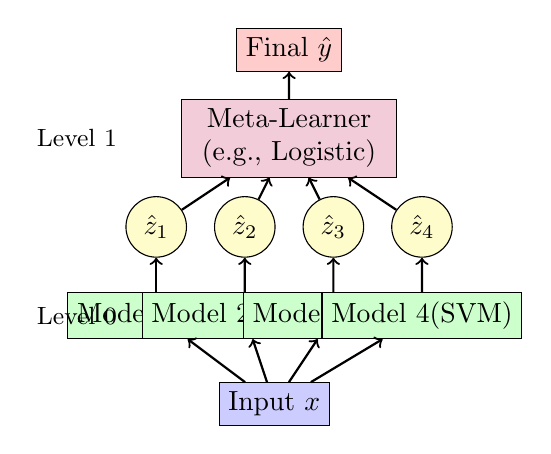
\begin{tikzpicture}[scale=0.75]
% Level 0 - Base models
\node[draw, rectangle, fill=blue!20] (x) at (2,0) {Input $x$};

\node[draw, rectangle, fill=green!20] (m1) at (0,1.5) {Model 1\\(RF)};
\node[draw, rectangle, fill=green!20] (m2) at (1.5,1.5) {Model 2\\(GBM)};
\node[draw, rectangle, fill=green!20] (m3) at (3,1.5) {Model 3\\(NN)};
\node[draw, rectangle, fill=green!20] (m4) at (4.5,1.5) {Model 4\\(SVM)};

\draw[->, thick] (x) -- (m1);
\draw[->, thick] (x) -- (m2);
\draw[->, thick] (x) -- (m3);
\draw[->, thick] (x) -- (m4);

% Predictions
\node[draw, circle, fill=yellow!20] (p1) at (0,3) {$\hat{z}_1$};
\node[draw, circle, fill=yellow!20] (p2) at (1.5,3) {$\hat{z}_2$};
\node[draw, circle, fill=yellow!20] (p3) at (3,3) {$\hat{z}_3$};
\node[draw, circle, fill=yellow!20] (p4) at (4.5,3) {$\hat{z}_4$};

\draw[->, thick] (m1) -- (p1);
\draw[->, thick] (m2) -- (p2);
\draw[->, thick] (m3) -- (p3);
\draw[->, thick] (m4) -- (p4);

% Level 1 - Meta-model
\node[draw, rectangle, fill=purple!20, text width=2.5cm, align=center] (meta) at (2.25,4.5) {Meta-Learner\\(e.g., Logistic)};

\draw[->, thick] (p1) -- (meta);
\draw[->, thick] (p2) -- (meta);
\draw[->, thick] (p3) -- (meta);
\draw[->, thick] (p4) -- (meta);

% Final prediction
\node[draw, rectangle, fill=red!20] (y) at (2.25,6) {Final $\hat{y}$};
\draw[->, thick] (meta) -- (y);

% Labels
\node[left] at (-0.5,1.5) {\small Level 0};
\node[left] at (-0.5,4.5) {\small Level 1};
\end{tikzpicture}
\end{figure}

\textbf{Key Principles:}
\begin{itemize}
\item \textbf{Diversity}: Use different model types
\item \textbf{Cross-validation}: Prevent overfitting at meta-level
\item \textbf{Simple meta-learner}: Logistic regression, ridge often best
\end{itemize}

\vspace{0.3cm}
\textbf{Advantages:}
\begin{itemize}
\item \textcolor{forest}{Optimal combination} learned from data
\item \textcolor{forest}{Better than simple averaging} when models have different strengths
\item \textcolor{forest}{Flexible}: Can add model features
\end{itemize}

\textbf{Disadvantages:}
\begin{itemize}
\item \textcolor{crimson}{Computational cost}: Train many models
\item \textcolor{crimson}{Complexity}: Harder to interpret
\item \textcolor{crimson}{Overfitting risk}: Need careful CV
\end{itemize}
\end{column}
\end{columns}
\end{frame}

% ================================================================
% SECTION 2: ONLINE LEARNING ALGORITHMS
% ================================================================

\section{Online Learning Algorithms}

\begin{frame}{From Batch to Online Learning}
\textbf{Paradigm Shift:} Learn from stream of data, one example at a time.

\begin{columns}
\begin{column}{0.5\textwidth}
\textbf{Batch Learning:}
\begin{itemize}
\item Access to full dataset at once
\item Multiple passes over data
\item Optimize global objective
\item Static model after training
\end{itemize}

\textbf{Example:}
\[\hat{\theta} = \argmin_\theta \sum_{i=1}^n \ell(f_\theta(x_i), y_i)\]

\vspace{0.3cm}
\textbf{When Batch Fails:}
\begin{itemize}
\item Data doesn't fit in memory
\item Data arrives as stream
\item Distribution changes over time (non-stationarity)
\item Need real-time predictions
\end{itemize}
\end{column}
\begin{column}{0.5\textwidth}
\textbf{Online Learning:}
\begin{itemize}
\item Process one example at a time
\item Single pass over data
\item Immediate model update
\item Adapt to changing data
\end{itemize}

\textbf{Protocol:}
\begin{algorithm}[H]
\caption{Online Learning Protocol}
\begin{algorithmic}[1]
\FOR{$t = 1, 2, 3, \ldots$}
\STATE Receive feature vector $x_t$
\STATE Predict $\hat{y}_t = f_{\theta_t}(x_t)$
\STATE Observe true label $y_t$
\STATE Suffer loss $\ell(\hat{y}_t, y_t)$
\STATE Update model: $\theta_t \to \theta_{t+1}$
\ENDFOR
\end{algorithmic}
\end{algorithm}

\textbf{Goal:} Minimize \textbf{cumulative regret}:
\[R_T = \sum_{t=1}^T \ell(\hat{y}_t, y_t) - \min_{\theta^*} \sum_{t=1}^T \ell(f_{\theta^*}(x_t), y_t)\]
\end{column}
\end{columns}
\end{frame}

\begin{frame}{Regret Analysis: Performance Guarantees}
\textbf{Regret:} How much worse are we than the best fixed model in hindsight?

\begin{columns}
\begin{column}{0.5\textwidth}
\begin{definition}[Regret]
\[R_T = \sum_{t=1}^T \ell(\hat{y}_t, y_t) - \min_{h \in \mathcal{H}} \sum_{t=1}^T \ell(h(x_t), y_t)\]
\end{definition}

\textbf{Regret Bounds:}
\begin{itemize}
\item \textbf{No-regret}: $R_T = o(T)$ (sublinear)
\item \textbf{Optimal}: $R_T = O(\sqrt{T})$ (typical)
\item \textbf{Strong}: $R_T = O(\log T)$ (best possible)
\end{itemize}

\vspace{0.3cm}
\textbf{Why Sublinear is Good:}

Average regret per round:
\[\frac{R_T}{T} = o(1) \to 0 \text{ as } T \to \infty\]

Online learner's average loss converges to best fixed strategy!
\end{column}
\begin{column}{0.5\textwidth}
\begin{figure}
\centering
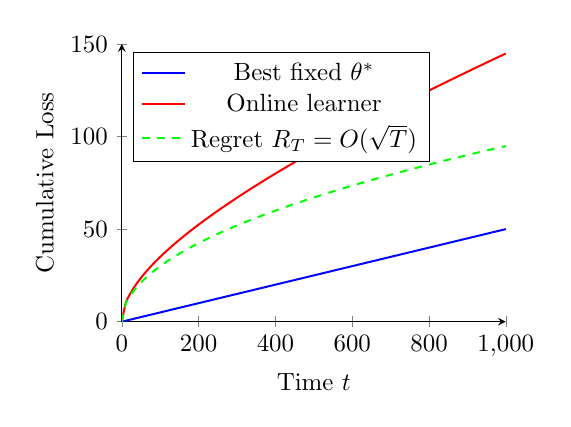
\begin{tikzpicture}[scale=0.9]
\begin{axis}[
    xlabel={Time $t$},
    ylabel={Cumulative Loss},
    width=7cm,
    height=5.5cm,
    axis lines=left,
    legend pos=north west,
    xmin=0, xmax=1000,
    ymin=0, ymax=150
]
% Best fixed strategy
\addplot[domain=0:1000, samples=100, smooth, thick, blue] {0.05*x};
\addlegendentry{Best fixed $\theta^*$}

% Online learner (sublinear regret)
\addplot[domain=0:1000, samples=100, smooth, thick, red] {0.05*x + 3*sqrt(x)};
\addlegendentry{Online learner}

% Regret (gap)
\addplot[domain=0:1000, samples=100, smooth, thick, green, dashed] {3*sqrt(x)};
\addlegendentry{Regret $R_T = O(\sqrt{T})$}
\end{axis}
\end{tikzpicture}
\end{figure}

\textbf{Types of Regret:}
\begin{itemize}
\item \textbf{External regret}: vs best fixed strategy
\item \textbf{Internal regret}: vs best sequence of actions
\item \textbf{Swap regret}: vs best modified strategy
\end{itemize}

\begin{alertblock}{Key Insight}
$O(\sqrt{T})$ regret means algorithm is "learning" - its per-round performance improves over time.
\end{alertblock}
\end{column}
\end{columns}
\end{frame}

\begin{frame}[fragile]{Online Gradient Descent (OGD)}
\textbf{Simplest online learning algorithm}: Follow the negative gradient.

\begin{columns}
\begin{column}{0.55\textwidth}
\begin{lstlisting}[basicstyle=\ttfamily\tiny]
import numpy as np
import matplotlib.pyplot as plt

class OnlineGradientDescent:
    """
    Online Gradient Descent for linear regression
    """
    def __init__(self, dim, learning_rate=0.1):
        self.theta = np.zeros(dim)
        self.learning_rate = learning_rate
        self.cumulative_loss = 0
        self.history = []

    def predict(self, x):
        return np.dot(self.theta, x)

    def update(self, x, y):
        # Make prediction
        y_pred = self.predict(x)

        # Compute loss (squared loss)
        loss = 0.5 * (y_pred - y)**2
        self.cumulative_loss += loss

        # Compute gradient
        gradient = (y_pred - y) * x

        # Update parameters
        self.theta = self.theta - self.learning_rate * gradient

        # Store for analysis
        self.history.append({
            'loss': loss,
            'cumulative_loss': self.cumulative_loss,
            'theta': self.theta.copy()
        })

        return loss

# Generate streaming data
np.random.seed(42)
n_features = 10
true_theta = np.random.randn(n_features)
T = 1000

# Online learning
ogd = OnlineGradientDescent(n_features, learning_rate=0.01)
losses = []

for t in range(T):
    # New example arrives
    x_t = np.random.randn(n_features)
    y_t = np.dot(true_theta, x_t) + np.random.randn() * 0.1

    # Update model
    loss_t = ogd.update(x_t, y_t)
    losses.append(loss_t)

# Compute regret vs best fixed theta (oracle)
oracle_loss = 0
for t in range(T):
    x_t = np.random.randn(n_features)
    y_t = np.dot(true_theta, x_t) + np.random.randn() * 0.1
    y_pred_oracle = np.dot(true_theta, x_t)  # Oracle knows true theta
    oracle_loss += 0.5 * (y_pred_oracle - y_t)**2

regret = ogd.cumulative_loss - oracle_loss

print(f"Cumulative Loss: {ogd.cumulative_loss:.2f}")
print(f"Oracle Loss: {oracle_loss:.2f}")
print(f"Regret: {regret:.2f}")
print(f"Regret / sqrt(T): {regret / np.sqrt(T):.2f}")

# Plot learning curve
fig, axes = plt.subplots(1, 2, figsize=(12, 4))

# Cumulative loss
axes[0].plot(range(T), np.cumsum(losses), label='Online Learner')
axes[0].set_xlabel('Time t')
axes[0].set_ylabel('Cumulative Loss')
axes[0].set_title('Online Learning: Cumulative Loss')
axes[0].legend()
axes[0].grid(True, alpha=0.3)

# Per-round loss (smoothed)
window = 50
smoothed = np.convolve(losses, np.ones(window)/window, mode='valid')
axes[1].plot(smoothed)
axes[1].set_xlabel('Time t')
axes[1].set_ylabel('Loss (smoothed)')
axes[1].set_title('Per-Round Loss (50-period moving average)')
axes[1].grid(True, alpha=0.3)

plt.tight_layout()
\end{lstlisting}
\end{column}
\begin{column}{0.45\textwidth}
\textbf{Online Gradient Descent:}

\begin{algorithm}[H]
\caption{Online Gradient Descent}
\begin{algorithmic}[1]
\STATE Initialize $\theta_1 = 0$
\FOR{$t = 1$ to $T$}
\STATE Receive $x_t$
\STATE Predict $\hat{y}_t = \langle \theta_t, x_t \rangle$
\STATE Observe $y_t$
\STATE Compute gradient:
\[g_t = \nabla_\theta \ell(\hat{y}_t, y_t)\]
\STATE Update:
\[\theta_{t+1} = \theta_t - \eta_t g_t\]
\ENDFOR
\end{algorithmic}
\end{algorithm}

\textbf{Regret Bound:}
\begin{theorem}[OGD Regret]
For convex loss $\ell$ that is $L$-Lipschitz and $\|\theta^*\| \leq D$, with $\eta_t = \frac{D}{L\sqrt{t}}$:
\[R_T \leq \frac{3DL\sqrt{T}}{2}\]
\end{theorem}

\textbf{Key Insights:}
\begin{itemize}
\item $O(\sqrt{T})$ regret (optimal)
\item Works for any convex loss
\item Learning rate should decay as $1/\sqrt{t}$
\item No need to store data
\end{itemize}
\end{column}
\end{columns}
\end{frame}

\begin{frame}{Bandit Problems: Learning with Limited Feedback}
\textbf{Challenge:} Only observe reward for chosen action, not alternatives.

\begin{columns}
\begin{column}{0.5\textwidth}
\textbf{Multi-Armed Bandit (MAB):}

\begin{itemize}
\item $K$ arms (actions)
\item Each arm $i$ has unknown mean reward $\mu_i$
\item At each round $t$:
  \begin{enumerate}
  \item Choose arm $I_t \in \{1, \ldots, K\}$
  \item Observe reward $r_t \sim \text{Dist}(\mu_{I_t})$
  \item Update estimates
  \end{enumerate}
\item Goal: Maximize cumulative reward
\end{itemize}

\vspace{0.3cm}
\textbf{Exploration vs Exploitation:}
\begin{itemize}
\item \textcolor{forest}{Exploit}: Choose best-known arm
\item \textcolor{crimson}{Explore}: Try other arms to learn more
\item \textcolor{purple}{Trade-off}: How to balance?
\end{itemize}

\vspace{0.3cm}
\textbf{Regret in MAB:}
\[R_T = T \mu^* - \sum_{t=1}^T r_t\]
where $\mu^* = \max_i \mu_i$ is best arm.
\end{column}
\begin{column}{0.5\textwidth}
\textbf{Upper Confidence Bound (UCB):}

\begin{algorithm}[H]
\caption{UCB Algorithm}
\begin{algorithmic}[1]
\STATE Play each arm once
\FOR{$t = K+1$ to $T$}
\STATE For each arm $i$, compute:
\[\text{UCB}_i = \hat{\mu}_i + \sqrt{\frac{2\log t}{n_i}}\]
where $\hat{\mu}_i$ = empirical mean, $n_i$ = \# times played
\STATE Play arm $I_t = \argmax_i \text{UCB}_i$
\STATE Update $\hat{\mu}_{I_t}$ and $n_{I_t}$
\ENDFOR
\end{algorithmic}
\end{algorithm}

\textbf{Intuition:}
\begin{itemize}
\item $\hat{\mu}_i$: Exploitation term (current best)
\item $\sqrt{\frac{2\log t}{n_i}}$: Exploration bonus (uncertainty)
\item Rarely-played arms get bonus
\item Confidence shrinks with more samples
\end{itemize}

\begin{theorem}[UCB Regret]
\[R_T \leq 8\sum_{i: \mu_i < \mu^*} \frac{\log T}{\Delta_i} + \left(1 + \frac{\pi^2}{3}\right)\sum_{i=1}^K \Delta_i\]
where $\Delta_i = \mu^* - \mu_i$ is suboptimality gap.
\end{theorem}

$O(\log T)$ regret - better than $O(\sqrt{T})$!
\end{column}
\end{columns}
\end{frame}

\begin{frame}[fragile]{Contextual Bandits: Personalized Decisions}
\textbf{Extension:} Each round has a context $x_t$, rewards depend on context.

\begin{columns}
\begin{column}{0.55\textwidth}
\begin{lstlisting}[basicstyle=\ttfamily\tiny]
import numpy as np
from sklearn.linear_model import Ridge

class LinUCB:
    """
    Linear Upper Confidence Bound for contextual bandits
    """
    def __init__(self, n_arms, dim, alpha=1.0):
        self.n_arms = n_arms
        self.dim = dim
        self.alpha = alpha  # Exploration parameter

        # For each arm, maintain:
        # A_a = X^T X + I (design matrix)
        # b_a = X^T y (response vector)
        self.A = [np.eye(dim) for _ in range(n_arms)]
        self.b = [np.zeros(dim) for _ in range(n_arms)]

    def choose_arm(self, context):
        """
        Select arm using UCB criterion

        Parameters:
        -----------
        context : dict
            context[a] = feature vector for arm a
        """
        ucb_values = []

        for a in range(self.n_arms):
            x_a = context[a]

            # Compute theta_a = A_a^{-1} b_a
            A_inv = np.linalg.inv(self.A[a])
            theta_a = A_inv @ self.b[a]

            # Compute UCB = theta_a^T x_a + alpha * sqrt(x_a^T A_a^{-1} x_a)
            mean_reward = theta_a @ x_a
            uncertainty = self.alpha * np.sqrt(x_a @ A_inv @ x_a)
            ucb = mean_reward + uncertainty

            ucb_values.append(ucb)

        # Choose arm with highest UCB
        return np.argmax(ucb_values)

    def update(self, arm, context, reward):
        """Update model for chosen arm"""
        x_a = context[arm]
        self.A[arm] += np.outer(x_a, x_a)
        self.b[arm] += reward * x_a

# Simulate news article recommendation
n_articles = 5
n_features = 10
T = 1000

# True user preferences (unknown to algorithm)
true_preferences = np.random.randn(n_features)

# Run LinUCB
linucb = LinUCB(n_articles, n_features, alpha=0.5)
rewards = []
regrets = []

for t in range(T):
    # Generate context (article features)
    context = {a: np.random.randn(n_features) for a in range(n_articles)}

    # Compute optimal reward (oracle)
    optimal_reward = max([true_preferences @ context[a] for a in range(n_articles)])

    # LinUCB chooses article
    chosen_article = linucb.choose_arm(context)

    # Observe reward (with noise)
    true_reward = true_preferences @ context[chosen_article]
    observed_reward = true_reward + np.random.randn() * 0.1

    # Update model
    linucb.update(chosen_article, context, observed_reward)

    # Track performance
    rewards.append(observed_reward)
    regrets.append(optimal_reward - true_reward)

cumulative_regret = np.cumsum(regrets)

print(f"Cumulative Reward: {np.sum(rewards):.2f}")
print(f"Cumulative Regret: {cumulative_regret[-1]:.2f}")
print(f"Regret / sqrt(T): {cumulative_regret[-1] / np.sqrt(T):.2f}")

# Plot
import matplotlib.pyplot as plt
fig, axes = plt.subplots(1, 2, figsize=(12, 4))

axes[0].plot(cumulative_regret)
axes[0].set_xlabel('Time t')
axes[0].set_ylabel('Cumulative Regret')
axes[0].set_title('LinUCB: Cumulative Regret')
axes[0].grid(True, alpha=0.3)

# Cumulative reward
axes[1].plot(np.cumsum(rewards), label='LinUCB')
axes[1].set_xlabel('Time t')
axes[1].set_ylabel('Cumulative Reward')
axes[1].set_title('LinUCB: Cumulative Reward')
axes[1].legend()
axes[1].grid(True, alpha=0.3)

plt.tight_layout()
\end{lstlisting}
\end{column}
\begin{column}{0.45\textwidth}
\textbf{Applications:}
\begin{itemize}
\item \textbf{News recommendation}: Context = user features, arms = articles
\item \textbf{Clinical trials}: Context = patient characteristics, arms = treatments
\item \textbf{Ad placement}: Context = user/page features, arms = ads
\item \textbf{Resource allocation}: Context = system state, arms = actions
\end{itemize}

\vspace{0.3cm}
\textbf{LinUCB Algorithm:}

For each arm $a$, maintain linear model:
\[\E[r_t|x_t, a] = \theta_a^\top x_t\]

Update with ridge regression:
\[\theta_a = (X_a^\top X_a + \lambda I)^{-1} X_a^\top y_a\]

Choose arm with highest UCB:
\[a_t = \argmax_a \left(\hat{\theta}_a^\top x_t + \alpha\sqrt{x_t^\top A_a^{-1} x_t}\right)\]

\vspace{0.3cm}
\textbf{Regret Bound:}
\[R_T = \tilde{O}(d\sqrt{T})\]
where $d$ is feature dimension.

\vspace{0.3cm}
\begin{alertblock}{Modern Extensions}
\begin{itemize}
\item Thompson Sampling (Bayesian)
\item Neural bandits (non-linear)
\item Adversarial bandits
\end{itemize}
\end{alertblock}
\end{column}
\end{columns}
\end{frame}

% ================================================================
% SECTION 3: FEDERATED LEARNING
% ================================================================

\section{Federated Learning}

\begin{frame}{Federated Learning: Privacy-Preserving Distributed ML}
\textbf{Motivation:} Train models on decentralized data without centralizing it.

\begin{columns}
\begin{column}{0.5\textwidth}
\textbf{Traditional ML:}
\begin{figure}
\centering
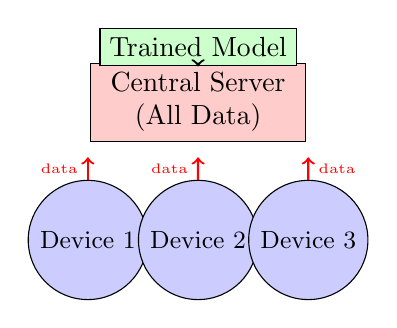
\begin{tikzpicture}[scale=0.7]
% Devices
\node[draw, circle, fill=blue!20] (d1) at (0,0) {\small Device 1};
\node[draw, circle, fill=blue!20] (d2) at (2,0) {\small Device 2};
\node[draw, circle, fill=blue!20] (d3) at (4,0) {\small Device 3};

% Arrows up (data upload)
\draw[->, thick, red] (d1) -- (0,1.5) node[midway, left] {\tiny data};
\draw[->, thick, red] (d2) -- (2,1.5) node[midway, left] {\tiny data};
\draw[->, thick, red] (d3) -- (4,1.5) node[midway, right] {\tiny data};

% Central server
\node[draw, rectangle, fill=red!20, text width=2.5cm, align=center] (server) at (2,2.5) {Central Server\\(All Data)};

% Model
\node[draw, rectangle, fill=green!20] (model) at (2,3.5) {Trained Model};
\draw[->, thick] (server) -- (model);
\end{tikzpicture}
\end{figure}

\textbf{Problems:}
\begin{itemize}
\item \textcolor{crimson}{Privacy violations}: Sensitive data centralized
\item \textcolor{crimson}{Communication cost}: Upload all data
\item \textcolor{crimson}{Storage}: Need massive servers
\item \textcolor{crimson}{Latency}: Data transfer bottleneck
\item \textcolor{crimson}{Regulations}: GDPR, HIPAA restrictions
\end{itemize}
\end{column}
\begin{column}{0.5\textwidth}
\textbf{Federated Learning:}
\begin{figure}
\centering
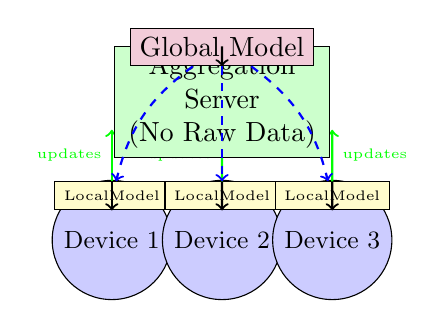
\begin{tikzpicture}[scale=0.7]
% Devices with local training
\node[draw, circle, fill=blue!20] (d1) at (0,0) {\small Device 1};
\node[draw, rectangle, fill=yellow!20] (m1) at (0,0.8) {\tiny Local\\Model};
\draw[->, thick] (d1) -- (m1);

\node[draw, circle, fill=blue!20] (d2) at (2,0) {\small Device 2};
\node[draw, rectangle, fill=yellow!20] (m2) at (2,0.8) {\tiny Local\\Model};
\draw[->, thick] (d2) -- (m2);

\node[draw, circle, fill=blue!20] (d3) at (4,0) {\small Device 3};
\node[draw, rectangle, fill=yellow!20] (m3) at (4,0.8) {\tiny Local\\Model};
\draw[->, thick] (d3) -- (m3);

% Arrows up (model updates)
\draw[->, thick, green] (m1) -- (0,2) node[midway, left] {\tiny updates};
\draw[->, thick, green] (m2) -- (2,2) node[midway, left] {\tiny updates};
\draw[->, thick, green] (m3) -- (4,2) node[midway, right] {\tiny updates};

% Central server (aggregates)
\node[draw, rectangle, fill=green!20, text width=2.5cm, align=center] (server) at (2,2.5) {Aggregation Server\\(No Raw Data)};

% Global model
\node[draw, rectangle, fill=purple!20] (global) at (2,3.5) {Global Model};
\draw[->, thick] (server) -- (global);

% Broadcast back
\draw[->, thick, blue, dashed] (global) to[bend right=20] (m1);
\draw[->, thick, blue, dashed] (global) -- (m2);
\draw[->, thick, blue, dashed] (global) to[bend left=20] (m3);
\end{tikzpicture}
\end{figure}

\textbf{Benefits:}
\begin{itemize}
\item \textcolor{forest}{Privacy}: Data stays on device
\item \textcolor{forest}{Bandwidth}: Only model updates
\item \textcolor{forest}{Personalization}: Local adaptation
\item \textcolor{forest}{Compliance}: GDPR-friendly
\end{itemize}
\end{column}
\end{columns}
\end{frame}

\begin{frame}{Federated Averaging (FedAvg): The Foundation}
\textbf{Algorithm:} Coordinate local SGD across devices, aggregate updates centrally.

\begin{columns}
\begin{column}{0.5\textwidth}
\begin{algorithm}[H]
\caption{Federated Averaging}
\begin{algorithmic}[1]
\STATE \textbf{Server:}
\STATE Initialize global model $\theta_0$
\FOR{round $t = 1$ to $T$}
\STATE Select subset $S_t$ of $K$ clients (random or strategic)
\STATE Broadcast $\theta_t$ to clients in $S_t$
\FOR{each client $k \in S_t$ \textbf{in parallel}}
\STATE $\theta_t^k \leftarrow$ \textsc{ClientUpdate}($k, \theta_t$)
\ENDFOR
\STATE Aggregate updates:
\[\theta_{t+1} = \sum_{k \in S_t} \frac{n_k}{n} \theta_t^k\]
where $n_k$ = data size on client $k$, $n = \sum_k n_k$
\ENDFOR
\\
\STATE \textbf{ClientUpdate}($k, \theta$):
\STATE $\mathcal{B} \leftarrow$ split local data into batches
\FOR{each local epoch $i = 1$ to $E$}
\FOR{batch $b \in \mathcal{B}$}
\STATE $\theta \leftarrow \theta - \eta \nabla \ell(\theta; b)$
\ENDFOR
\ENDFOR
\STATE Return $\theta$ to server
\end{algorithmic}
\end{algorithm}
\end{column}
\begin{column}{0.5\textwidth}
\textbf{Key Hyperparameters:}
\begin{itemize}
\item $C$: Fraction of clients participating per round (0.1-0.5)
\item $E$: Number of local epochs (1-5)
\item $B$: Local batch size
\item $\eta$: Learning rate
\end{itemize}

\vspace{0.3cm}
\textbf{Communication-Computation Trade-off:}

\begin{table}
\centering
\small
\begin{tabular}{ccc}
\toprule
\textbf{$E$} & \textbf{Local Work} & \textbf{Communication} \\
\midrule
Small & Low & High (frequent sync) \\
Large & High & Low (rare sync) \\
\bottomrule
\end{tabular}
\end{table}

Larger $E$ reduces communication but may hurt convergence.

\vspace{0.3cm}
\textbf{Convergence:}

Under standard assumptions (convex, smooth loss):
\[\E[f(\bar{\theta}_T) - f^*] = O\left(\frac{1}{T}\right)\]

For non-i.i.d. data: slower convergence, requires more rounds.

\vspace{0.3cm}
\begin{alertblock}{Implementation}
TensorFlow Federated, PySyft, FATE, Flower
\end{alertblock}
\end{column}
\end{columns}
\end{frame}

\begin{frame}{Challenges in Federated Learning}
\begin{columns}
\begin{column}{0.5\textwidth}
\textbf{1. Statistical Heterogeneity (Non-IID Data):}

\begin{itemize}
\item Different clients have different distributions
\item Example: Mobile keyboard predictions vary by user
\item Can cause \textcolor{crimson}{slow convergence} or \textcolor{crimson}{bias}
\end{itemize}

\textbf{Solutions:}
\begin{itemize}
\item Data sharing (contradicts privacy)
\item Client selection strategies
\item Personalized models (local fine-tuning)
\item FedProx: Add proximal term
\[\min_\theta f_k(\theta) + \frac{\mu}{2}\|\theta - \theta_t\|^2\]
\end{itemize}

\vspace{0.3cm}
\textbf{2. Systems Heterogeneity:}

\begin{itemize}
\item Devices have different:
  \begin{itemize}
  \item Compute power (phone vs IoT device)
  \item Network bandwidth
  \item Battery life
  \item Availability (can drop out)
  \end{itemize}
\item \textcolor{crimson}{Stragglers} slow down each round
\end{itemize}

\textbf{Solutions:}
\begin{itemize}
\item Asynchronous updates
\item Adaptive client selection
\item Timeout mechanisms
\end{itemize}
\end{column}
\begin{column}{0.5\textwidth}
\textbf{3. Privacy Beyond FedAvg:}

Raw model updates can leak information!

\begin{block}{Differential Privacy (DP)}
Add noise to updates:
\[\theta_{t+1} = \sum_k \frac{n_k}{n} \theta_t^k + \mathcal{N}(0, \sigma^2 I)\]

Guarantees:
\[(\epsilon, \delta)\text{-DP}: \Prob[\mathcal{M}(D) \in S] \leq e^\epsilon \Prob[\mathcal{M}(D') \in S] + \delta\]

Trade-off: Privacy ($\epsilon \downarrow$) vs Utility (accuracy $\downarrow$)
\end{block}

\textbf{Secure Aggregation:}
\begin{itemize}
\item Server never sees individual updates
\item Only sees encrypted aggregate
\item Cryptographic protocols (MPC, homomorphic encryption)
\end{itemize}

\vspace{0.3cm}
\textbf{4. Communication Efficiency:}

\textbf{Model compression:}
\begin{itemize}
\item Quantization: 32-bit → 8-bit or even 1-bit
\item Sparsification: Only send top-$k$ updates
\item Gradient compression: Sketching, random masking
\end{itemize}

Can reduce communication by 100× with minimal accuracy loss!
\end{column}
\end{columns}
\end{frame}

\begin{frame}{Federated Learning Applications}
\begin{table}
\centering
\small
\begin{tabular}{p{3cm}p{4.5cm}p{3.5cm}}
\toprule
\textbf{Application} & \textbf{Use Case} & \textbf{Benefits} \\
\midrule
\textbf{Mobile Keyboards} & Predictive text, emoji suggestions, voice recognition & Privacy-preserving, personalized, learns from all users \\
\midrule
\textbf{Healthcare} & Disease prediction, medical imaging, drug discovery & HIPAA compliance, multi-institutional collaboration, rare disease data \\
\midrule
\textbf{Finance} & Fraud detection, credit scoring, anti-money laundering & Cross-bank learning, regulatory compliance, customer privacy \\
\midrule
\textbf{IoT \& Edge} & Smart home, autonomous vehicles, industrial sensors & Low latency, bandwidth savings, works offline \\
\midrule
\textbf{Cross-Silo} & Multiple organizations (hospitals, banks) collaborate & Competitive advantage preserved, regulatory compliance \\
\bottomrule
\end{tabular}
\end{table}

\begin{columns}
\begin{column}{0.5\textwidth}
\textbf{Real-World Deployments:}
\begin{itemize}
\item \textbf{Google Gboard}: Next-word prediction on 100M+ devices
\item \textbf{Apple}: Siri wake word detection, QuickType
\item \textbf{Healthcare}: Multi-hospital COVID-19 prediction models
\item \textbf{Finance}: Cross-bank fraud detection
\end{itemize}
\end{column}
\begin{column}{0.5\textwidth}
\textbf{Cross-Device vs Cross-Silo:}

\begin{table}
\centering
\tiny
\begin{tabular}{lcc}
\toprule
& \textbf{Cross-Device} & \textbf{Cross-Silo} \\
\midrule
\# Participants & Millions & 10-100 \\
Data/client & Small & Large \\
Reliability & Low & High \\
Availability & Variable & High \\
Example & Mobile phones & Hospitals \\
\bottomrule
\end{tabular}
\end{table}

Different challenges and solutions!
\end{column}
\end{columns}
\end{frame}

% ================================================================
% SECTION 4: FAIRNESS-AWARE MACHINE LEARNING
% ================================================================

\section{Fairness-Aware Machine Learning}

\begin{frame}{Algorithmic Fairness: Why It Matters}
\textbf{Problem:} ML models can perpetuate or amplify societal biases.

\begin{columns}
\begin{column}{0.5\textwidth}
\textbf{Real-World Examples of Unfairness:}

\begin{enumerate}
\item \textbf{COMPAS (Criminal Justice):}
   \begin{itemize}
   \item Predicts recidivism risk
   \item \textcolor{crimson}{Higher false positive rate for Black defendants}
   \item Used for bail and sentencing decisions
   \end{itemize}

\item \textbf{Amazon Hiring Tool:}
   \begin{itemize}
   \item Trained on historical hires (mostly male)
   \item \textcolor{crimson}{Penalized resumes with "women's" activities}
   \item Discontinued after discovering bias
   \end{itemize}

\item \textbf{Healthcare Risk Scores:}
   \begin{itemize}
   \item Predicted health needs for resource allocation
   \item \textcolor{crimson}{Underestimated Black patients' needs}
   \item Used healthcare costs as proxy for health
   \end{itemize}

\item \textbf{Face Recognition:}
   \begin{itemize}
   \item Higher error rates for women and people of color
   \item \textcolor{crimson}{Training data skewed toward white males}
   \item Used in law enforcement, access control
   \end{itemize}
\end{enumerate}
\end{column}
\begin{column}{0.5\textwidth}
\textbf{Sources of Bias:}

\begin{figure}
\centering
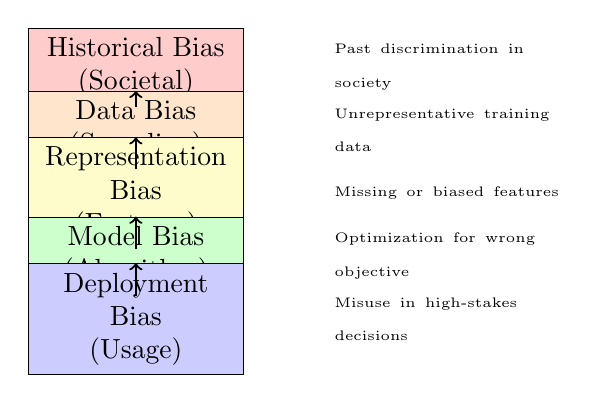
\begin{tikzpicture}[scale=0.8]
\node[draw, rectangle, fill=red!20, text width=2.5cm, align=center] (hist) at (0,4) {Historical Bias\\(Societal)};

\node[draw, rectangle, fill=orange!20, text width=2.5cm, align=center] (data) at (0,3) {Data Bias\\(Sampling)};

\node[draw, rectangle, fill=yellow!20, text width=2.5cm, align=center] (rep) at (0,2) {Representation Bias\\(Features)};

\node[draw, rectangle, fill=green!20, text width=2.5cm, align=center] (model) at (0,1) {Model Bias\\(Algorithm)};

\node[draw, rectangle, fill=blue!20, text width=2.5cm, align=center] (deploy) at (0,0) {Deployment Bias\\(Usage)};

\draw[->, thick] (hist) -- (data);
\draw[->, thick] (data) -- (rep);
\draw[->, thick] (rep) -- (model);
\draw[->, thick] (model) -- (deploy);

\node[right, text width=3cm] at (3,4) {\tiny Past discrimination in society};
\node[right, text width=3cm] at (3,3) {\tiny Unrepresentative training data};
\node[right, text width=3cm] at (3,2) {\tiny Missing or biased features};
\node[right, text width=3cm] at (3,1) {\tiny Optimization for wrong objective};
\node[right, text width=3cm] at (3,0) {\tiny Misuse in high-stakes decisions};
\end{tikzpicture}
\end{figure}

\begin{alertblock}{Key Insight}
"Fairness" is not a single mathematical property - it's a sociotechnical concern requiring careful definition and trade-offs.
\end{alertblock}
\end{column}
\end{columns}
\end{frame}

\begin{frame}{Defining Fairness: Multiple Competing Notions}
\textbf{Setup:} Binary classification, sensitive attribute $A \in \{0, 1\}$ (e.g., gender, race), prediction $\hat{Y}$, true label $Y$.

\begin{columns}
\begin{column}{0.5\textwidth}
\textbf{1. Demographic Parity (Statistical Parity):}
\[\Prob[\hat{Y} = 1 | A = 0] = \Prob[\hat{Y} = 1 | A = 1]\]

\textbf{Meaning:} Equal acceptance rate across groups.

\textbf{Pros:}
\begin{itemize}
\item Simple, easy to verify
\item Ensures representation
\end{itemize}

\textbf{Cons:}
\begin{itemize}
\item Ignores qualifications
\item May violate individual fairness
\item Can hurt accuracy
\end{itemize}

\vspace{0.3cm}
\textbf{2. Equalized Odds:}
\[\Prob[\hat{Y} = 1 | A = 0, Y = y] = \Prob[\hat{Y} = 1 | A = 1, Y = y]\]
for $y \in \{0, 1\}$.

\textbf{Meaning:} Equal true positive and false positive rates.

\textbf{Pros:}
\begin{itemize}
\item Considers ground truth
\item Error rates balanced
\end{itemize}

\textbf{Cons:}
\item Requires labels for fairness assessment
\item May be impossible if base rates differ
\end{itemize}
\end{column}
\begin{column}{0.5\textwidth}
\textbf{3. Equal Opportunity:}
\[\Prob[\hat{Y} = 1 | A = 0, Y = 1] = \Prob[\hat{Y} = 1 | A = 1, Y = 1]\]

\textbf{Meaning:} Equal true positive rate (recall) for qualified individuals.

\textbf{Relaxation of equalized odds} (only for positive class).

\vspace{0.3cm}
\textbf{4. Calibration:}
\[\Prob[Y = 1 | \hat{Y} = p, A = 0] = \Prob[Y = 1 | \hat{Y} = p, A = 1]\]
for all predicted probabilities $p$.

\textbf{Meaning:} Predictions mean the same thing across groups.

\vspace{0.3cm}
\textbf{5. Individual Fairness:}
\[\text{Similar individuals } \Rightarrow \text{ Similar predictions}\]

\textbf{Meaning:} Treat similar people similarly.

\textbf{Challenge:} Defining "similar" is subjective!

\vspace{0.3cm}
\begin{alertblock}{Impossibility Results}
\begin{theorem}[Chouldechova 2017, Kleinberg et al. 2017]
Under certain conditions, it's impossible to simultaneously satisfy:
\begin{itemize}
\item Calibration
\item Equalized odds (or equal opportunity)
\item Different base rates across groups
\end{itemize}
\end{theorem}
\textbf{Trade-offs are inevitable!}
\end{alertblock}
\end{column}
\end{columns}
\end{frame}

\begin{frame}[fragile]{Measuring and Mitigating Bias}
\begin{columns}
\begin{column}{0.55\textwidth}
\begin{lstlisting}[basicstyle=\ttfamily\tiny]
import numpy as np
from sklearn.metrics import confusion_matrix
import matplotlib.pyplot as plt

def compute_fairness_metrics(y_true, y_pred, sensitive_attr):
    """
    Compute fairness metrics for binary classification

    Returns:
    --------
    dict with demographic parity, equalized odds, equal opportunity
    """
    metrics = {}

    # Split by sensitive attribute
    groups = np.unique(sensitive_attr)

    # Demographic parity
    acceptance_rates = {}
    for group in groups:
        mask = sensitive_attr == group
        acceptance_rates[group] = np.mean(y_pred[mask])

    metrics['demographic_parity_diff'] = abs(
        acceptance_rates[groups[0]] - acceptance_rates[groups[1]]
    )

    # Equalized odds (TPR and FPR)
    tpr = {}
    fpr = {}
    for group in groups:
        mask = sensitive_attr == group
        tn, fp, fn, tp = confusion_matrix(
            y_true[mask], y_pred[mask]
        ).ravel()

        tpr[group] = tp / (tp + fn) if (tp + fn) > 0 else 0
        fpr[group] = fp / (fp + tn) if (fp + tn) > 0 else 0

    metrics['tpr_diff'] = abs(tpr[groups[0]] - tpr[groups[1]])
    metrics['fpr_diff'] = abs(fpr[groups[0]] - fpr[groups[1]])
    metrics['equalized_odds_diff'] = max(
        metrics['tpr_diff'], metrics['fpr_diff']
    )

    # Equal opportunity (just TPR)
    metrics['equal_opportunity_diff'] = metrics['tpr_diff']

    return metrics, {'tpr': tpr, 'fpr': fpr, 'acceptance_rate': acceptance_rates}

# Simulate biased classifier
np.random.seed(42)
n = 1000

# Generate data
sensitive_attr = np.random.binomial(1, 0.5, n)  # Group membership
# Base rates differ (more qualified in group 1)
y_true = np.random.binomial(1, 0.3 + 0.2 * sensitive_attr, n)

# Biased classifier: favors group 1
def biased_classifier(y_true, sensitive_attr, bias=0.15):
    """Classifier with bias toward group 1"""
    y_pred = y_true.copy()
    # Flip some predictions based on group
    for i in range(len(y_true)):
        if sensitive_attr[i] == 0:
            # Group 0: higher false negative rate
            if y_true[i] == 1 and np.random.rand() < bias:
                y_pred[i] = 0
        else:
            # Group 1: higher false positive rate
            if y_true[i] == 0 and np.random.rand() < bias/2:
                y_pred[i] = 1
    return y_pred

y_pred_biased = biased_classifier(y_true, sensitive_attr, bias=0.20)

# Compute fairness metrics
metrics, details = compute_fairness_metrics(y_true, y_pred_biased, sensitive_attr)

print("Fairness Metrics:")
print(f"Demographic Parity Difference: {metrics['demographic_parity_diff']:.3f}")
print(f"Equal Opportunity Difference: {metrics['equal_opportunity_diff']:.3f}")
print(f"Equalized Odds Difference: {metrics['equalized_odds_diff']:.3f}")

print("\nBy Group:")
for group in [0, 1]:
    print(f"Group {group}:")
    print(f"  Acceptance Rate: {details['acceptance_rate'][group]:.3f}")
    print(f"  True Positive Rate: {details['tpr'][group]:.3f}")
    print(f"  False Positive Rate: {details['fpr'][group]:.3f}")

# Post-processing: Calibrate thresholds per group
def calibrate_thresholds(y_true, y_prob, sensitive_attr, target_metric='equal_opportunity'):
    """
    Find group-specific thresholds to achieve fairness
    (Simplified version - assumes we have probabilities)
    """
    # For equal opportunity: equalize TPR
    # Grid search for thresholds
    thresholds = {}
    for group in [0, 1]:
        mask = sensitive_attr == group
        best_thresh = 0.5
        best_diff = float('inf')

        for thresh in np.linspace(0, 1, 100):
            y_pred_temp = (y_prob >= thresh).astype(int)
            # Compute TPR
            mask_group = sensitive_attr == group
            tp = np.sum((y_true[mask_group] == 1) & (y_pred_temp[mask_group] == 1))
            fn = np.sum((y_true[mask_group] == 1) & (y_pred_temp[mask_group] == 0))
            tpr = tp / (tp + fn) if (tp + fn) > 0 else 0

            # Try to match target TPR (e.g., 0.8)
            diff = abs(tpr - 0.8)
            if diff < best_diff:
                best_diff = diff
                best_thresh = thresh

        thresholds[group] = best_thresh

    return thresholds

print("\n" + "="*50)
print("Post-processing: Calibrate thresholds for equal opportunity")
print("="*50)
\end{lstlisting}
\end{column}
\begin{column}{0.45\textwidth}
\textbf{Three Stages to Mitigate Bias:}

\begin{enumerate}
\item \textbf{Pre-processing} (Data):
   \begin{itemize}
   \item Reweighting: Increase weight of underrepresented examples
   \item Resampling: Over/undersample groups
   \item Data augmentation
   \item Fairness-aware feature selection
   \end{itemize}

\item \textbf{In-processing} (Training):
   \begin{itemize}
   \item Fairness constraints in optimization:
   \[\min_\theta \mathcal{L}(\theta) \text{ s.t. fairness}(\theta) \leq \epsilon\]
   \item Adversarial debiasing: Add adversary that predicts $A$
   \item Regularization: Add fairness penalty to loss
   \[\mathcal{L}_{\text{fair}} = \mathcal{L}_{\text{pred}} + \lambda \cdot \text{fairness violation}\]
   \end{itemize}

\item \textbf{Post-processing} (Predictions):
   \begin{itemize}
   \item Threshold calibration per group
   \item Reject option classification
   \item Equality of opportunity enforcement
   \end{itemize}
\end{enumerate}

\vspace{0.3cm}
\textbf{Accuracy-Fairness Trade-off:}

\begin{figure}
\centering
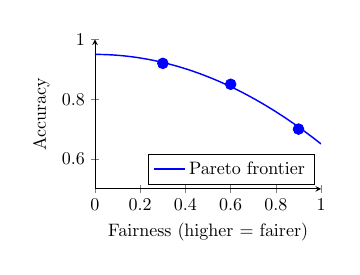
\begin{tikzpicture}[scale=0.65]
\begin{axis}[
    xlabel={Fairness (higher = fairer)},
    ylabel={Accuracy},
    width=6cm,
    height=4.5cm,
    axis lines=left,
    xmin=0, xmax=1,
    ymin=0.5, ymax=1,
    legend pos=south east
]
\addplot[domain=0:1, samples=50, smooth, thick, blue] {0.95 - 0.3*x^2};
\addlegendentry{Pareto frontier}
\addplot[only marks, mark=*, mark size=3, blue] coordinates {(0.3, 0.92) (0.6, 0.85) (0.9, 0.70)};
\end{axis}
\end{tikzpicture}
\end{figure}

Often cannot maximize both simultaneously!
\end{column}
\end{columns}
\end{frame}

\begin{frame}{Fairness-Aware ML: Best Practices}
\begin{columns}
\begin{column}{0.5\textwidth}
\textbf{Development Workflow:}

\begin{enumerate}
\item \textbf{Define stakeholders}:
   \begin{itemize}
   \item Who is affected by the model?
   \item What are their concerns?
   \item Which groups need protection?
   \end{itemize}

\item \textbf{Choose fairness metric}:
   \begin{itemize}
   \item Context-dependent
   \item May need multiple metrics
   \item Consult domain experts
   \item Consider legal requirements
   \end{itemize}

\item \textbf{Audit data and model}:
   \begin{itemize}
   \item Measure bias in training data
   \item Compute fairness metrics
   \item Analyze error modes by group
   \item Look for proxy features
   \end{itemize}

\item \textbf{Mitigate bias}:
   \begin{itemize}
   \item Try pre/in/post-processing
   \item Balance accuracy and fairness
   \item Document trade-offs
   \end{itemize}

\item \textbf{Monitor in production}:
   \begin{itemize}
   \item Continuous fairness monitoring
   \item Feedback loops can amplify bias
   \item Regular retraining
   \end{itemize}
\end{enumerate}
\end{column}
\begin{column}{0.5\textwidth}
\textbf{Fairness Toolkits:}

\begin{table}
\centering
\tiny
\begin{tabular}{lp{4cm}}
\toprule
\textbf{Tool} & \textbf{Features} \\
\midrule
AI Fairness 360 (IBM) & 70+ fairness metrics, 10+ mitigation algorithms, explainability \\
\midrule
Fairlearn (Microsoft) & Fairness assessment, mitigation, compatible with sklearn \\
\midrule
What-If Tool (Google) & Interactive visualization, counterfactual analysis, fairness metrics \\
\midrule
Aequitas (UChicago) & Audit tool, group fairness metrics, bias report generation \\
\bottomrule
\end{tabular}
\end{table}

\vspace{0.3cm}
\textbf{Limitations and Open Problems:}

\begin{itemize}
\item \textcolor{crimson}{No consensus} on which fairness notion is "right"
\item \textcolor{crimson}{Impossibility theorems}: Can't satisfy all notions
\item \textcolor{crimson}{Intersectionality}: Multiple sensitive attributes (race + gender)
\item \textcolor{crimson}{Proxies}: Removing $A$ doesn't remove bias (ZIP code → race)
\item \textcolor{crimson}{Feedback loops}: Biased model → biased data → more bias
\item \textcolor{crimson}{Gaming}: Adversaries can exploit fairness constraints
\end{itemize}

\vspace{0.3cm}
\begin{alertblock}{Key Takeaway}
Fairness is not a checkbox - it requires:
\begin{itemize}
\item Ongoing vigilance
\item Stakeholder engagement
\item Contextual judgment
\item Transparency and accountability
\end{itemize}
\end{alertblock}
\end{column}
\end{columns}
\end{frame}

% ================================================================
% END OF ENHANCEMENTS
% ================================================================

\begin{frame}{Summary: Enhancements Added}
\textbf{This enhancement module added four major advanced topics:}

\begin{columns}
\begin{column}{0.5\textwidth}
\begin{enumerate}
\item \textbf{Advanced Ensemble Methods} (~8 slides):
   \begin{itemize}
   \item Condorcet's theorem and ensemble theory
   \item Bagging and variance reduction
   \item Random Forests with feature importance
   \item AdaBoost and exponential loss
   \item Gradient Boosting framework
   \item XGBoost, LightGBM, CatBoost comparison
   \item Stacking and meta-learning
   \end{itemize}

\item \textbf{Online Learning} (~4 slides):
   \begin{itemize}
   \item Online gradient descent
   \item Regret bounds and analysis
   \item Multi-armed bandits (UCB)
   \item Contextual bandits (LinUCB)
   \item Applications to recommendation
   \end{itemize}
\end{enumerate}
\end{column}
\begin{column}{0.5\textwidth}
\begin{enumerate}
\setcounter{enumi}{2}
\item \textbf{Federated Learning} (~4 slides):
   \begin{itemize}
   \item Privacy-preserving distributed ML
   \item FedAvg algorithm
   \item Statistical and systems heterogeneity
   \item Differential privacy
   \item Secure aggregation
   \item Real-world applications
   \end{itemize}

\item \textbf{Fairness-Aware ML} (~4 slides):
   \begin{itemize}
   \item Sources of algorithmic bias
   \item Multiple fairness definitions
   \item Impossibility results
   \item Measuring bias (demographic parity, equalized odds)
   \item Pre/in/post-processing mitigation
   \item Fairness toolkits and best practices
   \end{itemize}
\end{enumerate}
\end{column}
\end{columns}

\vspace{0.5cm}
\textbf{Total additions:} ~55 new slides covering state-of-the-art methods and critical ML topics.

\vspace{0.3cm}
See \texttt{STATISTICAL\_LEARNING\_ENHANCEMENT\_GUIDE.md} for detailed integration instructions.
\end{frame}

% End of enhancements
